%% \tableofcontents

\subsection{The CMS detector}\label{cms}

The CMS detector is fully described in \cite{DTperformance}. An schematic view of the CMS detector is shown in Figure~\ref{fig:CMS}.

\begin{figure}
\centering
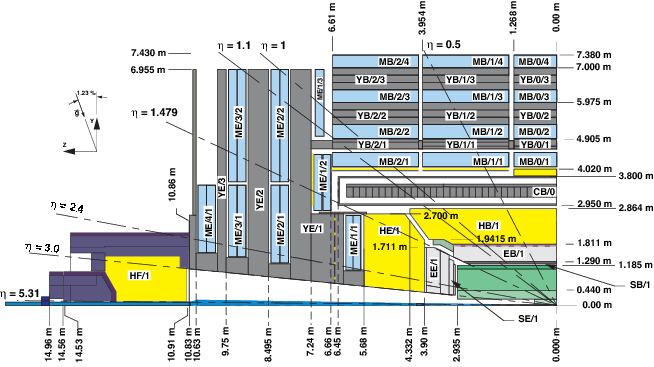
\includegraphics[width=0.45\textwidth]{figures/CMSview1.png}
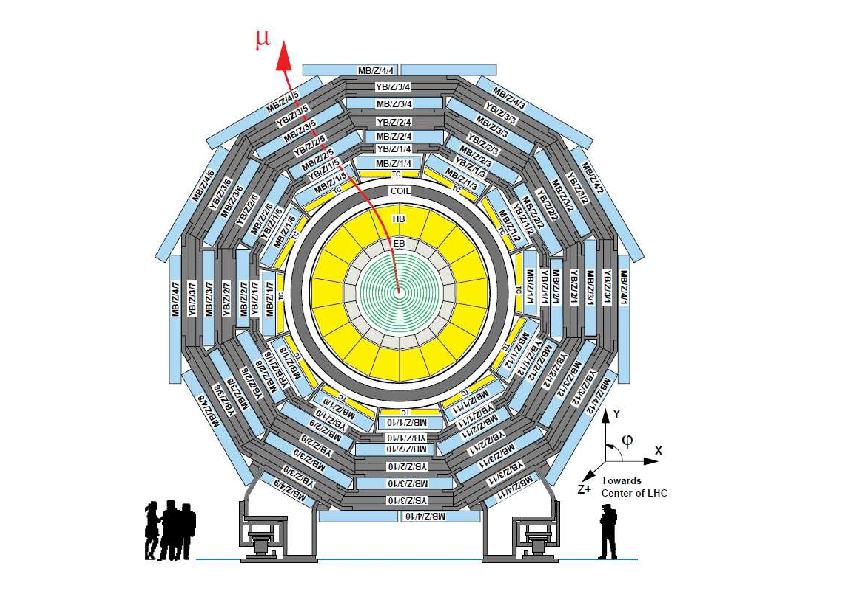
\includegraphics[width=0.45\textwidth]{figures/CMSview.png}
\caption{Schematic view of the CMS detector. Left: longitudinal view of one quarter of the detector. Right: transverse view at $z = 0$. Both figures have been taken from \cite{DTperformance}}
\label{fig:CMS}
\end{figure}



\subsection{Experimental challenges in high $p_{T}$ muon measurement}\label{challenges}

TEST

\subsection{The TuneP algorithm}\label{TuneP}

TEST
